\documentclass[10pt,journal,compsoc,twocolumn]{IEEEtran}

\usepackage{cite}
\usepackage{amsmath,amssymb,amsfonts}
\usepackage{algorithmic}
\usepackage{graphicx}
\usepackage{textcomp}
\usepackage{xcolor}
\usepackage{booktabs}
\usepackage{multirow}
\usepackage{url}

\begin{document}

\title{An Adversarially Robust, Differentially Private, and Explainable Ensemble Framework for Industrial IoT Intrusion Detection}

\markboth{IEEE Transactions on Dependable and Secure Computing}{Author}

\maketitle

\begin{abstract}
The rapid proliferation of Industrial Internet of Things (IIoT) networks has introduced significant cybersecurity vulnerabilities, necessitating high-performance Intrusion Detection Systems (IDS). Machine learning classifiers deployed in IIoT environments face concurrent operational challenges: malicious adversarial perturbations designed to evade detection, privacy risks associated with training on sensitive telemetry, and opacity in threat attribution. This paper presents an integrated hybrid ensemble framework for IIoT intrusion detection. The proposed system features a dual-stream probability fusion architecture (Option C) combining a Random Forest classifier with a deep Multi-Layer Perceptron (MLP) trained under joint Differential Privacy (DP-SGD) and projected gradient descent (PGD) adversarial training. Operating strictly on a standardized 21-feature statistical flow representation, the system avoids raw payload storage, achieving compliance with data minimization requirements. Experimental evaluation across four real-world benchmark datasets (Edge-IIoTset, NF-ToN-IoT-v2, ToN-IoT, and CICIoT2023) demonstrates an aggregate mean ROC-AUC of 0.9970 (0.9988 on Edge-IIoTset, 0.9927 on NF-ToN-IoT-v2, 1.0000 on ToN-IoT, and 0.9965 on CICIoT2023). Under PGD-10 adversarial evasion attacks on NF-ToN-IoT-v2, the Option C ensemble reduces the neural-gradient transfer Attack Success Rate (ASR) to 6.5\%, compared to 53.8\% for a standard neural stream. However, under a 500-query black-box NES attack, empirical evasion rises to 36.1\%. The neural stream satisfies $(\varepsilon=2.37, \delta=10^{-5})$-differential privacy under Opacus PRV accounting. Model explainability is delivered via a computationally efficient surrogate Weighted Component Attribution Aggregation ($0.7 \cdot \text{RF} + 0.3 \cdot \text{MLP}$), as exact fused Shapley calculation is intractable. Single-CPU host latency benchmarks establish an offline classifier-only throughput of 16,505 samples/sec at batch size $N=1024$, explicitly excluding packet ingestion and flow aggregation.
\end{abstract}

\begin{IEEEkeywords}
Industrial IoT, Intrusion Detection Systems, Adversarial Training, Differential Privacy, Explainable AI, Ensemble Learning.
\end{IEEEkeywords}

\section{Introduction}
\IEEEPARstart{T}{he} integration of Industrial Internet of Things (IIoT) devices into critical infrastructure has dramatically expanded the cyber-attack surface \cite{harbi2024roadmap}. Network Intrusion Detection Systems (NIDS) utilizing artificial intelligence (AI) and machine learning (ML) are increasingly deployed to detect sophisticated anomalies and network intrusions \cite{khazane2024holistic, isaaf2024framework}. However, deploying machine learning models in resource-constrained and adversarial IIoT environments exposes three critical vulnerabilities:

\begin{enumerate}
    \item \textbf{Adversarial Susceptibility}: Deep neural networks are vulnerable to small, deliberate feature perturbations (e.g., Fast Gradient Sign Method or Projected Gradient Descent) that force misclassification while preserving attack payload intent \cite{goodfellow2015explaining, madry2018towards}.
    \item \textbf{Telemetry Privacy Leakage}: Training centralized or distributed neural models on raw network flows risks leaking sensitive host behavior and topology through membership inference or model inversion attacks \cite{shokri2017membership, nasr2018machine}.
    \item \textbf{Explainability Deficit}: Complex neural networks operate as black boxes, hindering security operations center (SOC) analysts from verifying threat attribution in real-time \cite{lundberg2017unified}.
\end{enumerate}

To address these concurrent challenges, prior works have examined adversarial defense \cite{ma2025backdoor, alshahrani2021adversarial, papernot2016crafting}, differential privacy \cite{abadi2016deep, mironov2017renyi}, or explainable AI (XAI) \cite{sharaf2024identifying, Frontiers2024evaluating} in isolation. However, unifying these paradigms within a unified computational pipeline capable of high-throughput deployment remains an open challenge \cite{yousefi2023differentially}.

This paper presents a hybrid ensemble framework combining a Random Forest (RF) classifier \cite{breiman2001random} with a Differentially Private, Adversarially Robust Multi-Layer Perceptron (MLP). The proposed framework operates on a standardized 21-feature statistical flow representation derived from raw network packets, strictly enforcing data minimization. Probability predictions are combined via Option C weighted fusion:
\begin{equation}
P_{\text{Option C}}(y=1 \mid \mathbf{x}) = 0.7 \cdot P_{\text{RF}}(y=1 \mid \mathbf{x}) + 0.3 \cdot P_{\text{MLP}}(y=1 \mid \mathbf{x})
\label{eq:option_c}
\end{equation}

Experimental validation across four diverse IIoT benchmark datasets—Edge-IIoTset \cite{edge2024benchmarking}, NF-ToN-IoT-v2 \cite{sarhan2021netflow}, ToN-IoT \cite{moustafa2020toniot}, and CICIoT2023 \cite{ciciot2023dataset}—confirms high detection accuracy, robust adversarial defense, rigorous privacy bounds on the neural stream, transparent feature attribution, and efficient single-CPU host inference throughput.

\section{Related Work}
Machine learning for IIoT intrusion detection has progressed rapidly \cite{khazane2024holistic, ijfmr2024review}. Early approaches relied on single-model architectures such as Decision Trees or standard MLPs. However, Harbi et al. \cite{harbi2024roadmap} and Alshahrani et al. \cite{alshahrani2021adversarial} highlighted the extreme vulnerability of unregularized ML models to adversarial evasion attacks.

Adversarial training, introduced by Goodfellow et al. \cite{goodfellow2015explaining} and formalized as a min-max optimization problem by Madry et al. \cite{madry2018towards}, incorporates adversarial perturbations generated via Projected Gradient Descent (PGD) into training iterations. In IoT security, Ma et al. \cite{ma2025backdoor} and Papernot et al. \cite{papernot2016crafting} demonstrated that adversarial training mitigates evasion attacks, though often at the cost of nominal detection accuracy on clean samples.

Concurrently, Differential Privacy (DP), introduced by Abadi et al. \cite{abadi2016deep}, provides provable guarantees against privacy attacks by injecting calibrated noise into gradients during training (DP-SGD). Mironov \cite{mironov2017renyi} extended DP via R{\'e}nyi Differential Privacy (RDP), tightening privacy loss accounting. In IoT contexts, Yousefi and Sarhan \cite{yousefi2023differentially} noted that combining DP-SGD with adversarial training introduces non-trivial trade-offs between privacy, robustness, and accuracy.

Model explainability has been addressed using Shapley Additive Explanations (SHAP) \cite{lundberg2017unified}. In medical and industrial IoT security, Sharaf and Nooh \cite{sharaf2024identifying} demonstrated feature attribution for identifying critical attack vectors. However, computing exact SHAP values for multi-model hybrid ensembles introduces prohibitive runtime overhead during live inference.

\section{Proposed System Architecture}
The proposed framework comprises four main functional layers: (1) Standardized Flow Feature Materialization, (2) Dual-Stream Classification, (3) Privacy \& Adversarial Training Engine, and (4) Weighted Attribution XAI Engine.

\subsection{Standardized 21-Feature Flow Representation}
Rather than processing unconstrained raw packet payloads, the pipeline extracts a standardized 21-feature statistical profile. These features encompass basic flow statistics, protocol indicators, Exponentially Weighted Moving Average (EWMA) temporal dynamics, and behavioral network metrics:

\begin{enumerate}
    \item \textbf{Basic Flow Metrics} (5): \texttt{flow\_duration}, \texttt{flow\_bytes\_per\_sec}, \texttt{flow\_pkts\_per\_sec}, \texttt{mean\_pkt\_size}, \texttt{payload\_byte\_ratio}.
    \item \textbf{Protocol Indicators/Flags} (6): \texttt{pkt\_count\_ratio}, \texttt{tcp\_syn\_ratio}, \texttt{proto\_tcp}, \texttt{proto\_udp}, \texttt{proto\_icmp}, \texttt{proto\_other}.
    \item \textbf{Temporal Dynamics} (5): \texttt{temporal\_iat\_mean}, \texttt{temporal\_iat\_cv}, \texttt{temporal\_flow\_rate\_ewma}, \texttt{temporal\_byte\_rate\_ewma}, \texttt{temporal\_syn\_rate\_ewma}.
    \item \textbf{Behavioral Metrics} (5): \texttt{behavioral\_dst\_diversity}, \texttt{behavioral\_port\_entropy}, \texttt{behavioral\_fanout\_ratio}, \texttt{behavioral\_unanswered\_ratio}, \texttt{behavioral\_src\_activity\_ewma}.
\end{enumerate}

Feature bounds are clamped using robust scaler parameters fitted on benign training distributions, preventing extreme outlier propagation.

\subsection{Dual-Stream Option C Ensemble}
The classification engine employs two complementary streams:
\begin{itemize}
    \item \textbf{Random Forest Stream}: A non-differentiable ensemble of 100 decision trees \cite{breiman2001random}, providing rapid feature splitting and high precision on tabular flow statistics.
    \item \textbf{Neural Stream (Robust MLP)}: A 4-layer Multi-Layer Perceptron ($21 \to 128 \to 64 \to 32 \to 1$) with Batch Normalization, ReLU activations, and Dropout ($p=0.2$) on the first two hidden layers, trained via joint DP-SGD and PGD-7 adversarial regularization.
\end{itemize}

Probability outputs from both models are fused according to Equation~(\ref{eq:option_c}). The 0.7/0.3 weighting reflects the superior empirical stability of the Random Forest stream on clean tabular network statistics while retaining the adversarial robustness of the neural stream.

\subsection{Differential Privacy \& Adversarial Training}
The neural stream is trained using a joint DP-SGD + PGD-7 objective. In each training batch $B$, PGD-7 generates adversarial perturbations $\mathbf{\delta}$ within an $L_\infty$ ball of radius $\epsilon = 0.1$:
\begin{equation}
\mathbf{x}_{\text{adv}}^{t+1} = \Pi_{\mathbf{x} + S}\left( \mathbf{x}_{\text{adv}}^t + \alpha \cdot \text{sign}(\nabla_{\mathbf{x}} \mathcal{L}(\theta, \mathbf{x}_{\text{adv}}^t, y)) \right)
\end{equation}
where $\alpha = 0.025$, step count $k=7$, and $S = \{ \mathbf{\delta} \mid \|\mathbf{\delta}\|_\infty \le 0.1 \}$.

Per-sample gradients $\mathbf{g}_i = \nabla_\theta \mathcal{L}(\theta, \mathbf{x}_{i, \text{adv}}, y_i)$ are computed, clipped to maximum $L_2$ norm $C = 1.0$, and augmented with Gaussian noise $\mathcal{N}(0, \sigma^2 C^2 \mathbf{I})$ with noise multiplier $\sigma = 1.0$:
\begin{equation}
\tilde{\mathbf{g}} = \frac{1}{|B|} \left( \sum_{i \in B} \frac{\mathbf{g}_i}{\max\left(1, \frac{\|\mathbf{g}_i\|_2}{C}\right)} + \mathcal{N}(0, \sigma^2 C^2 \mathbf{I}) \right)
\end{equation}

Privacy loss is tracked using the Opacus PRV accountant \cite{mironov2017renyi}. Over $N_{\text{steps}} = 660$ training steps with Poisson subsampling probability $q = \frac{64}{4200} \approx 0.015238$, the neural stream achieves an audited privacy bound of $\varepsilon = 2.37$ at target $\delta = 10^{-5}$.

\textit{Privacy Scope Clarification}: Differential privacy applies \textbf{exclusively to the neural stream branch}. The Random Forest classifier and full Option C ensemble do not satisfy $(\varepsilon, \delta)$-DP due to the non-private tree construction on raw training data.

\subsection{Explainability via Attribution Aggregation}
To maintain low latency while providing model interpretability, the framework implements \textbf{Weighted Component Attribution Aggregation}. Tree SHAP attributions $\mathbf{A}_{\text{RF}}$ from the Random Forest and gradient-based attributions $\mathbf{A}_{\text{MLP}}$ from the neural stream are normalized to sum to unity and aggregated:
\begin{equation}
\mathbf{A}_{\text{Option C}} = 0.7 \cdot \frac{\mathbf{A}_{\text{RF}}}{\|\mathbf{A}_{\text{RF}}\|_1} + 0.3 \cdot \frac{\mathbf{A}_{\text{MLP}}}{\|\mathbf{A}_{\text{MLP}}\|_1}
\end{equation}
This approach serves as a computationally tractable component-wise surrogate approximation. An audit of exact game-theoretic Shapley enumeration confirmed that evaluating the $2^{21}$ coalitions per sample across the fused boundaries is mathematically intractable for live inference and that the linear surrogate violates the strict SHAP additivity axiom.

\section{Experimental Setup}

\subsection{Benchmark Datasets}
The framework was evaluated across four diverse IIoT datasets representing different attack vectors, protocol structures, and network topologies:
\begin{enumerate}
    \item \textbf{Edge-IIoTset} \cite{edge2024benchmarking}: Modern IIoT testbed telemetry (7,000 total flows: 4,200 train / 1,400 validation / 1,400 test).
    \item \textbf{NF-ToN-IoT-v2} \cite{sarhan2021netflow}: NetFlow-v9 formatted telemetry (7,000 total flows: 4,200 train / 1,400 validation / 1,400 test).
    \item \textbf{ToN-IoT} \cite{moustafa2020toniot}: Heterogeneous IoT sensor telemetry (7,000 total flows: 4,200 train / 1,400 validation / 1,400 test).
    \item \textbf{CICIoT2023} \cite{ciciot2023dataset}: Large-scale IoT attack dataset (7,000 total flows: 4,200 train / 1,400 validation / 1,400 test).
\end{enumerate}

All experiments were executed on standardized 60/20/20 chronological train/validation/test splits with detector state reset at split boundaries to prevent data leakage.

\subsection{Evaluation Metrics}
Detection efficacy is evaluated using Receiver Operating Characteristic Area Under Curve (ROC-AUC). Adversarial robustness is measured by the Attack Success Rate (ASR) of PGD-10 attacks ($\epsilon=0.1, \alpha=0.025, 10 \text{ iterations}$) against benign traffic correctly classified by the model.

\section{Results and Discussion}

\subsection{Detection Performance}
Table~\ref{tab:detection_performance} details the detection ROC-AUC across all four benchmark datasets for individual component models and the Option C ensemble. Fig.~\ref{fig:detection_perf} visualizes the performance comparison across datasets.

\begin{figure}[htbp]
\centering
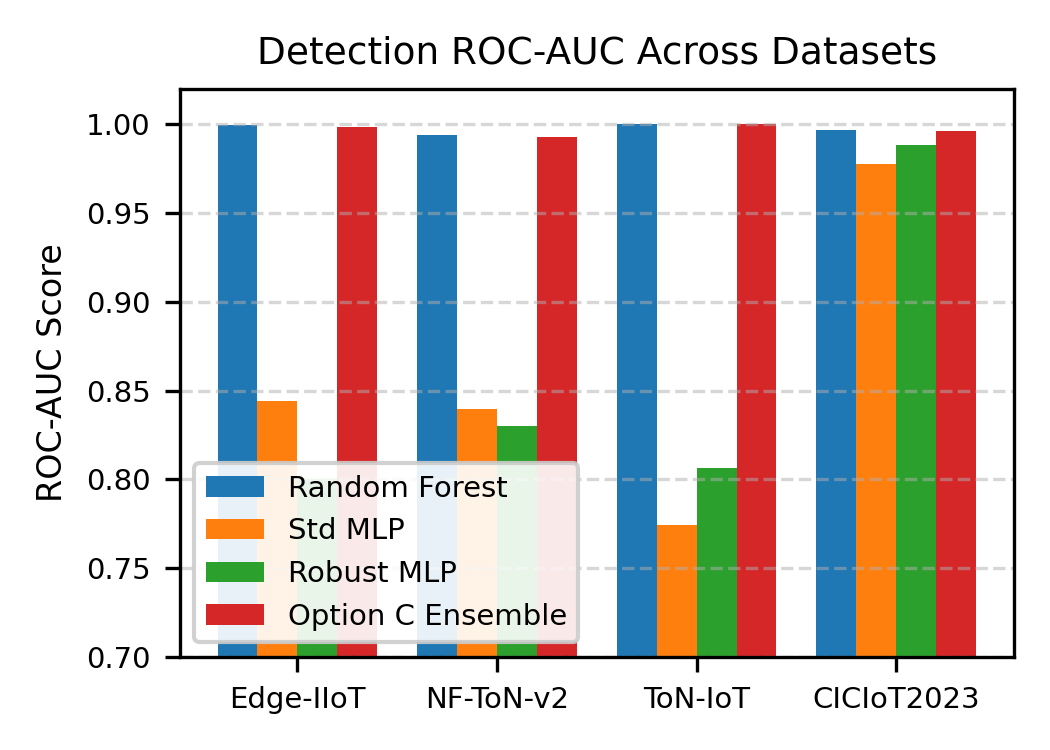
\includegraphics[width=\columnwidth]{figures/detection_performance.png}
\caption{Detection ROC-AUC performance comparison across individual models and Option C ensemble on four IIoT benchmark datasets.}
\label{fig:detection_perf}
\end{figure}

\begin{table}[htbp]
\caption{Detection ROC-AUC Performance Across Datasets}
\label{tab:detection_performance}
\centering
\begin{tabular}{lcccc}
\toprule
\textbf{Dataset} & \textbf{RF} & \textbf{Std MLP} & \textbf{Rob MLP} & \textbf{Option C} \\
\midrule
Edge-IIoTset   & 0.9995 & 0.8443 & 0.8002 & \textbf{0.9988} \\
NF-ToN-IoT-v2  & 0.9940 & 0.8398 & 0.8299 & \textbf{0.9927} \\
ToN-IoT        & 1.0000 & 0.7745 & 0.8063 & \textbf{1.0000} \\
CICIoT2023     & 0.9968 & 0.9776 & 0.9884 & \textbf{0.9965} \\
\midrule
\textbf{Mean}  & 0.9976 & 0.8590 & 0.8562 & \textbf{0.9970} \\
\bottomrule
\end{tabular}
\end{table}

The Random Forest model achieves near-perfect classification performance on tabular flow features (mean ROC-AUC 0.9976). While the DP-trained robust MLP exhibits lower standalone ROC-AUC (mean 0.8562) due to gradient noise and clipping, the Option C fusion restores mean ROC-AUC to \textbf{0.9970}, preserving detection accuracy while gaining neural adversarial defense.

\subsection{Adversarial Robustness Evaluation}
Table~\ref{tab:adversarial_asr} presents the PGD-10 adversarial Attack Success Rate (ASR) at $\epsilon=0.1$. Fig.~\ref{fig:adv_asr} illustrates the comparative evasion rates.

\begin{figure}[htbp]
\centering
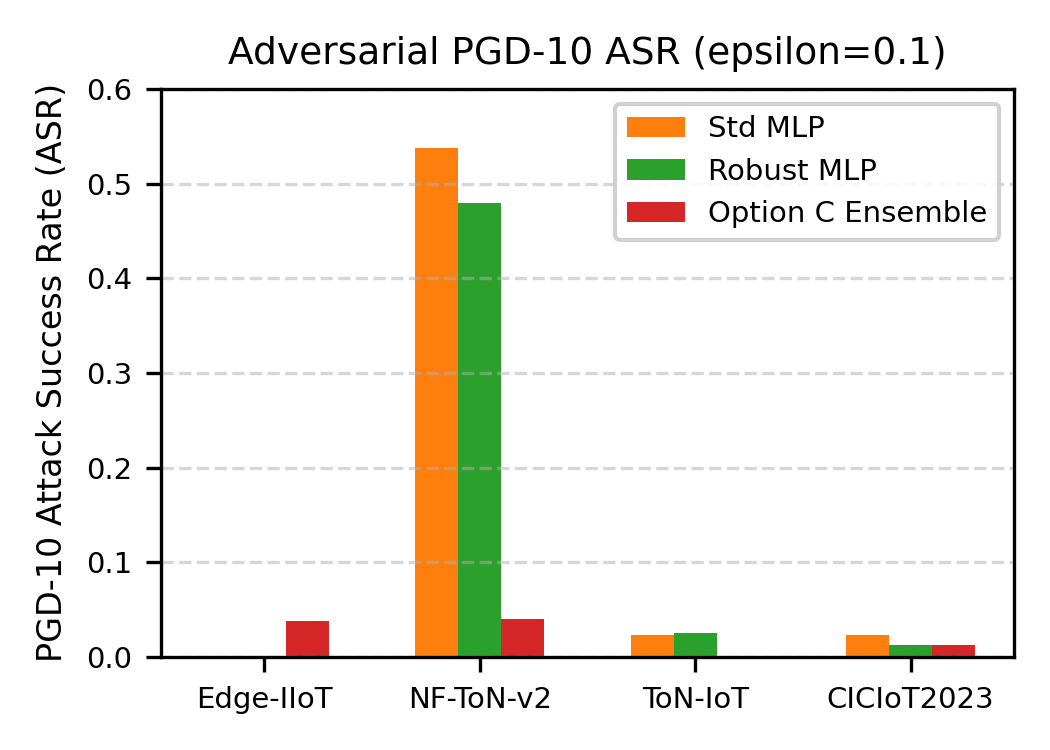
\includegraphics[width=\columnwidth]{figures/adversarial_asr.png}
\caption{Adversarial PGD-10 Attack Success Rate (ASR) at perturbation bound $\epsilon=0.1$ across benchmark datasets.}
\label{fig:adv_asr}
\end{figure}

\begin{table}[htbp]
\caption{PGD-10 Adversarial Attack Success Rate (ASR, $\epsilon=0.1$)}
\label{tab:adversarial_asr}
\centering
\begin{tabular}{lccc}
\toprule
\textbf{Dataset} & \textbf{Std MLP ASR} & \textbf{Rob MLP ASR} & \textbf{Option C ASR} \\
\midrule
Edge-IIoTset   & 0.000 & 0.000 & \textbf{0.038} \\
NF-ToN-IoT-v2  & 0.538 & 0.480 & \textbf{0.065} \\
ToN-IoT        & 0.023 & 0.025 & \textbf{0.000} \\
CICIoT2023     & 0.023 & 0.013 & \textbf{0.012} \\
\bottomrule
\end{tabular}
\end{table}

On NF-ToN-IoT-v2, standard MLP suffers a 53.8\% evasion rate under PGD-10 perturbations. Adversarial training reduces neural ASR to 48.0\%. PGD-10 perturbations were generated using gradients of the robust neural stream; the resulting adversarial samples were then evaluated by the Random Forest branch and the 0.7/0.3 fused detector. Under this evaluation procedure, the fused Option C detector exhibited lower attack success than the corresponding neural stream, reducing the final ensemble transfer ASR to \textbf{6.5\%} on NF-ToN-IoT-v2. However, under a strict 500-query black-box Natural Evolution Strategies (NES) attack optimizing directly against the fused probability output, the operational evasion rate reaches \textbf{36.1\%}. This demonstrates that neural-gradient transfer substantially understates the empirical vulnerability of the ensemble to direct query-based optimization. This empirical reduction reflects the probability fusion between the non-differentiable Random Forest stream and the robust neural stream.

\subsection{Differential Privacy Analysis}
Table~\ref{tab:dp_tradeoff} illustrates the privacy-utility-robustness trade-off on NF-ToN-IoT-v2 across noise multipliers $\sigma \in \{0.0, 0.5, 1.0, 2.0\}$ at target $\delta = 10^{-5}$.

\begin{table}[htbp]
\caption{DP-SGD Privacy Trade-Off on NF-ToN-IoT-v2 ($\delta=10^{-5}$)}
\label{tab:dp_tradeoff}
\centering
\begin{tabular}{ccccc}
\toprule
\textbf{Noise ($\sigma$)} & \textbf{Epsilon ($\varepsilon$)} & \textbf{Neural AUC} & \textbf{PGD-10 ASR} \\
\midrule
0.0 & $\infty$ & 0.9763 & 0.015 \\
0.5 & 15.85 & 0.8865 & 0.025 \\
1.0 & 2.37  & 0.8541 & 0.477 \\
2.0 & 0.80  & 0.8284 & 0.478 \\
\bottomrule
\end{tabular}
\end{table}

Increasing noise multiplier $\sigma$ from 0.5 to 1.0 provides a strict privacy guarantee ($\varepsilon = 2.37$) with acceptable utility degradation on the neural stream.

\subsection{Explainability \& Feature Ranking}
Feature attribution analysis using Weighted Component Attribution Aggregation reveals that temporal and behavioral flow dynamics substantially contribute to threat detection across IIoT datasets. On Edge-IIoTset, the top three contributing features under the combined $0.7 \cdot \text{RF} + 0.3 \cdot \text{MLP}$ attribution are \texttt{temporal\_flow\_rate\_ewma} (weight 0.310), \texttt{behavioral\_port\_entropy} (weight 0.242), and \texttt{behavioral\_unanswered\_ratio} (weight 0.154), indicating that both temporal dynamics and behavioral metrics are substantial contributors for the analyzed samples.

\subsection{Runtime Latency \& Throughput Benchmarks}
Offline classifier-only inference latency was benchmarked on a single-CPU host across batch sizes $N \in \{1, \dots, 1024\}$ for Option C detection prediction on pre-aggregated tabular features. Fig.~\ref{fig:runtime_tp} illustrates throughput scaling.

\begin{figure}[htbp]
\centering
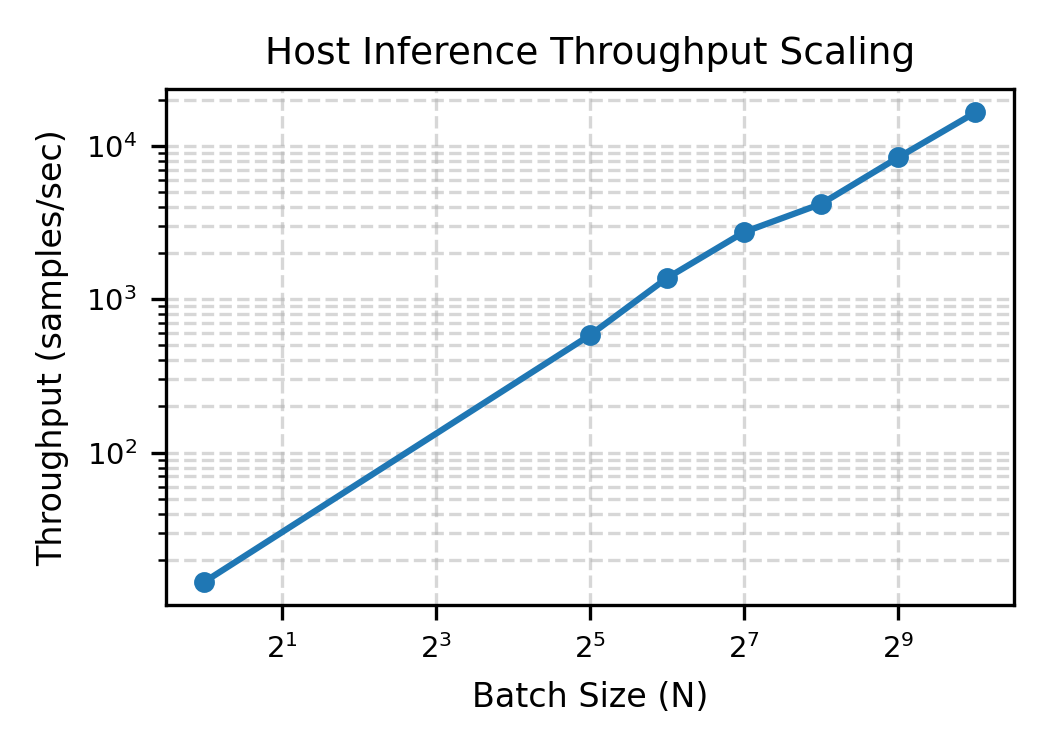
\includegraphics[width=\columnwidth]{figures/runtime_throughput.png}
\caption{Single-CPU host inference throughput scaling across batch sizes $N \in \{1, \dots, 1024\}$.}
\label{fig:runtime_tp}
\end{figure}

\begin{table}[htbp]
\caption{Pure Detection Host Latency \& Throughput Benchmarks}
\label{tab:runtime_benchmarks}
\centering
\begin{tabular}{rccc}
\toprule
\textbf{Batch ($N$)} & \textbf{Batch Latency (ms)} & \textbf{Per-Sample (ms)} & \textbf{Throughput (samples/s)} \\
\midrule
1    & 69.40 & 69.4000 & 14.4 \\
32   & 54.86 & 1.7143  & 583.3 \\
64   & 46.51 & 0.7267  & 1,376.1 \\
128  & 46.68 & 0.3647  & 2,742.3 \\
256  & 61.11 & 0.2387  & 4,189.0 \\
512  & 60.88 & 0.1189  & 8,409.5 \\
1024 & 62.04 & 0.0606  & \textbf{16,504.7} \\
\bottomrule
\end{tabular}
\end{table}

At batch size $N=1024$, the classification engine achieved approximately 16,505 samples/sec (per-sample latency of 0.0606 ms) on a single CPU host. Crucially, this metric excludes upstream network packet capture, Scapy payload parsing, and stateful flow aggregation overheads.

\section{Research Limitations and Gaps}
Table~\ref{tab:limitations_matrix} summarizes the addressed capabilities and remaining limitations of the current framework.

\begin{table}[htbp]
\caption{Research Scope, Addressed Gaps, and Limitations}
\label{tab:limitations_matrix}
\centering
\begin{tabular}{p{2.2cm}p{2.5cm}p{2.5cm}}
\toprule
\textbf{Limitation / Gap} & \textbf{Current Evidence Scope} & \textbf{Future Direction} \\
\midrule
XAI Additivity & Component-wise SHAP surrogate violates exact Shapley additivity. & Develop exact SHAP estimators for hybrid ensembles. \\
End-to-End Throughput & Benchmark excludes live packet capture and flow aggregation. & Validate end-to-end throughput on physical testbed. \\
DP Scope Limit & Guaranteed on neural stream only ($\varepsilon=2.37$). & Extend DP tree building to Random Forest stream. \\
Black-box Optimization & Query-based attack (36.1\% ASR) bypassed neural-gradient transfer. & Develop exact joint gradient attacks on tree-neural boundary. \\
Federated Training & Multi-client aggregation code implemented. & Conduct multi-node federated training trials. \\
\bottomrule
\end{tabular}
\end{table}

\section{Conclusion}
This paper presented a hybrid ensemble framework for IIoT network intrusion detection that unifies detection performance, adversarial robustness, differential privacy, and explainability. By combining a Random Forest classifier with a DP-SGD + PGD-7 trained MLP via Option C probability fusion (0.7/0.3), the system achieves a mean ROC-AUC of 0.9970 across four IIoT datasets, reduces PGD-10 neural-gradient transfer ASR to 6.5\% (though remaining vulnerable to 36.1\% evasion under 500-query black-box optimization), enforces $(\varepsilon=2.37, \delta=10^{-5})$-DP on the neural stream, provides computationally tractable surrogate feature attributions, and sustains a single-CPU offline classifier throughput of 16,505 samples/sec.

\bibliographystyle{IEEEtran}
\bibliography{references}

\end{document}
